\chapter{Исследовательский раздел}

\section{Предмет исследования}

Для проведения исследования работы реализованного метода хранения аудио-файлов в NoSQL-базе данных было составлено 9 MIDI-файлов, отличающихся только количеством музыкальных дорожек (MTrk). Таким образом, первый файл содержит одну музыкальную дорожку, второй - 2, ..., девятый - 9. Данные дорожек не отличаются, в зависимости от их количества незначительно меняется заголовок MIDI-файла: поля Format и NumTracks.
Так, например, аудио-файл, содержащий одну музыкальную дорожку, имеет в базе данных заголовок, представленный на рисунке 4.1.

\begin{center}
		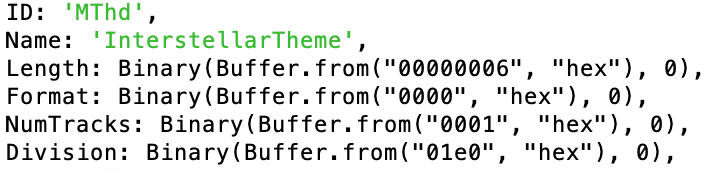
\includegraphics[scale=0.6]{tex/img/OneTrack.png}
		
			Рис 4.1 — Заголовок MIDI-файла, содержащего одну MTrk
\end{center}

Заголвок MIDI-файла с девятью дорожками представлен на рисунке 4.2.
\begin{center}
		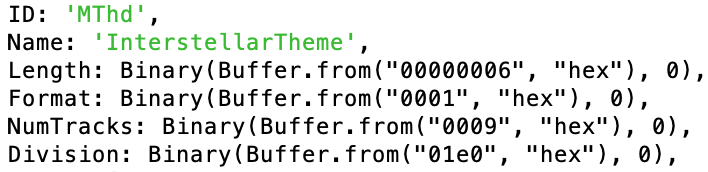
\includegraphics[scale=0.6]{tex/img/NineTracks.png}
		
			Рис 4.2 — Заголовок MIDI-файла, содержащего девять MTrk
\end{center}

Цель исследования - сравнить временные показатели работы с MIDI-файлом при реализованном методе хранения в MongoDB и при хранении его в базе данных в виде неструктурированного массива байтов. Исследуется работа методов хранения при следующих командах базы данных.
\begin{enumerate}
\item Только добавление документа в MongoDB.
\item Только извлечение документа из MongoDB (с последующим доступом к данным самой последней музыкальной дорожки).
\item Добавление и извлечение документа из MongoDB (с последующим доступом к данным самой последней музыкальной дорожки).
\end{enumerate}

В случае реализованного метода распределенного хранения MIDI-файлов, все девять файлов будут храниться в базе данных в виде специальной структуры. Сопоставляемый с ним метод предполагает хранение в виде документа, содержащего один элемент с полем Data, имеющим значение, равное массиву байтов, считанному из аудио-файла. На рисунке 4.3 приведен пример того, как в MongoDB будет представлен такой файл.

\begin{center}
		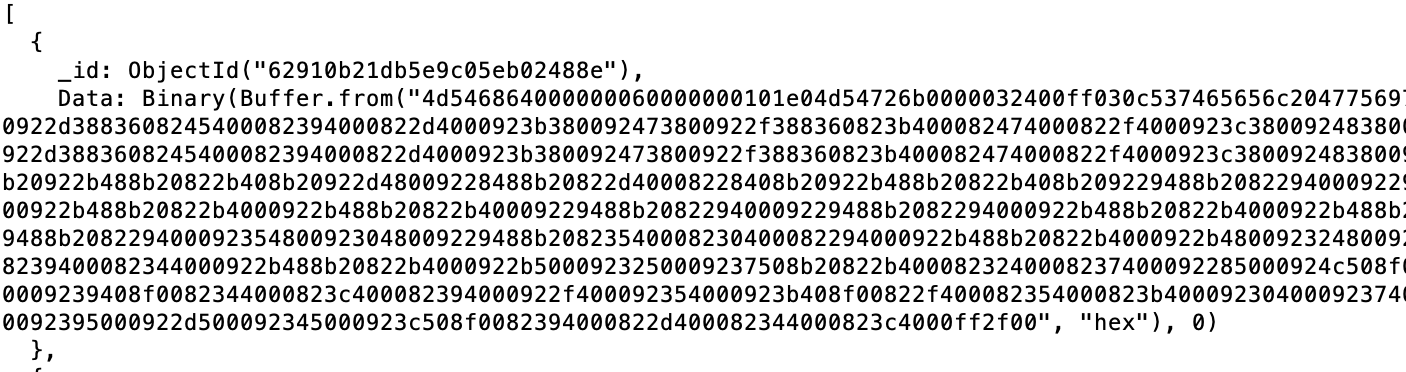
\includegraphics[scale=0.5]{tex/img/Bytes.png}
		
			Рис 4.3 — Метод хранения MIDI-файла в MongoDB в виде массива байтов
\end{center}

\section{Характеристики ЭВМ}

Для исследования использовалась ЭВМ со следующими характеристиками.
\begin{itemize}
	\item MacBook Pro (Retina, 15-inch, Mid 2014).
	\item 2,5 GHz Intel Core i7.
	\item Число логических ядер: 8.
\end{itemize}

\section{Результаты исследования}

\subsection{Добавление документа в MongoDB}

Для добавления MIDI-файла в базу данных для хранения в структурированном виде был реализован метод, формирующий документ MongoDB с помощью пути к аудио-файлу и его имени (листинг \ref{lst:insert_command_test1}). После инициализации документа созданный объект добавляется в базу данных.

\newpage

\begin{lstlisting}[language=C, label=some-code, caption=Добавление MIDI-файла в MongoDB c использованием реализованного метода, label=lst:insert_command_test1]
private async void AddDocument(string number, string name)
        {
            var document = new BsonDocument { { "path", "/Users/anastasia/Desktop/Audiofiles/Interstellar" + number + ".mid" }, 
                { "name", name } };
            _midiCollection.InsertOne(document);
        }
\end{lstlisting}

При вставке массива байтов аудио-файла он считывается из соответствующего файла в переменную array, которая используется для инициализации данных специального типа (бинарный массив) и формирования из них документа MongoDB. По завершении этих действий документ добавляется в базу данных (листинг \ref{lst:insert_command_test2}).

\begin{lstlisting}[language=C, label=some-code, caption=Добавление MIDI-файла в MongoDB в виде массива байтов, label=lst:insert_command_test2]
private async void AddBytesMongoDb(byte[] array)
        {
            var bsonBinaryData = new BsonBinaryData(array);
            var document = new BsonDocument(new BsonElement("Data", bsonBinaryData));
            _midiCollection.InsertOne(document);
        }
\end{lstlisting}

На рисунке 4.4 представлен результат работы методов хранения. Пояснения исследуемых характеристик приведены на рисунке 4.5.

\begin{center}
		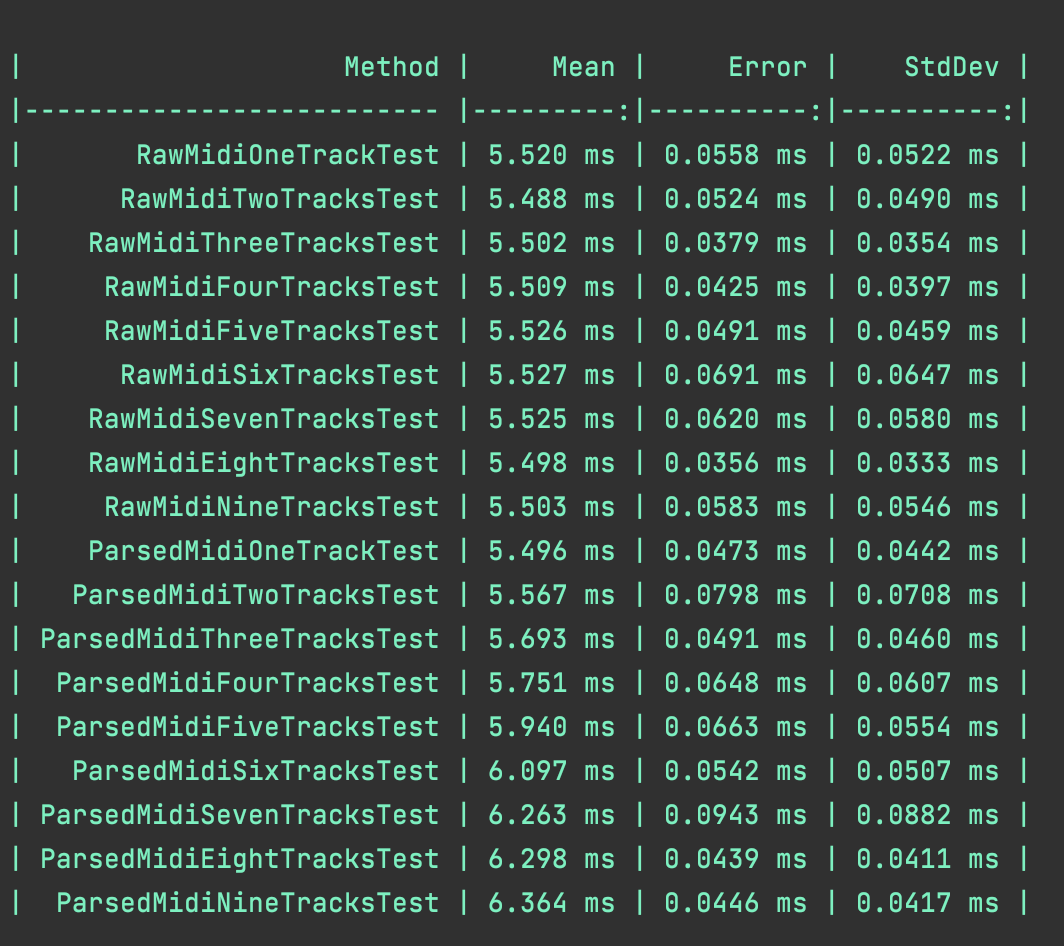
\includegraphics[scale=0.6]{tex/img/InsertClean.png}
		
			Рис 4.4 — Сводная таблица работы методов при добавлении в MongoDB
\end{center}

\begin{center}
		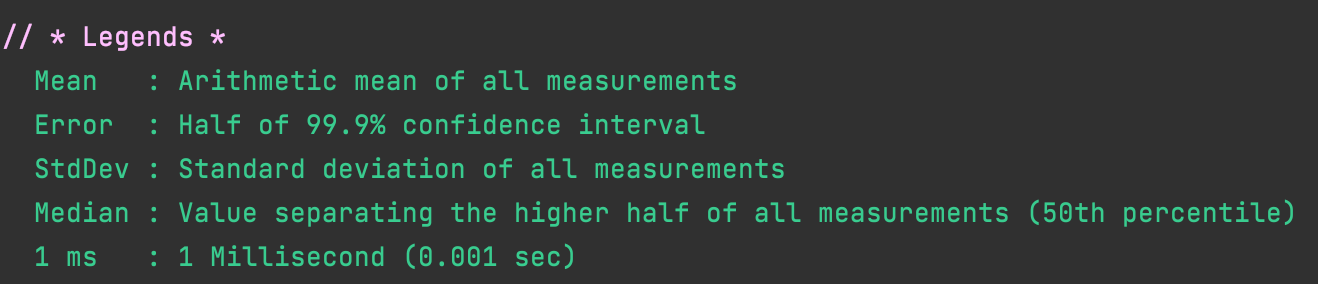
\includegraphics[scale=0.6]{tex/img/Legends.png}
		
			Рис 4.5 — Сводная таблица работы методов при добавлении в MongoDB
\end{center}

На рисунке 4.6 полученные временные характеристики представлены в графическом виде.

\begin{center}
		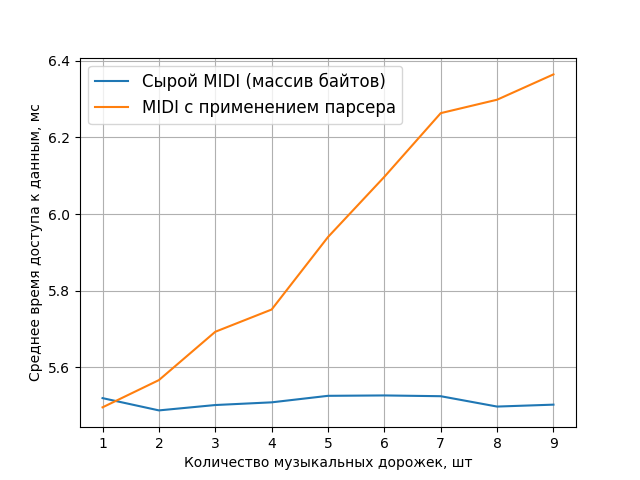
\includegraphics[scale=0.7]{tex/img/figure_insert_query.png}
		
			Рис 4.6 — Сравнение работы методов при добавлении в MongoDB
\end{center}

Как видно из рисунков 4.4 и 4.6, наибольшая скорость работы операции добавления документа в MongoDB достигается при использовании метода хранения MIDI-файла на основе его содержания. Однако, при увеличении количества музыкальных дорожек время работы этого метода растет пропорционально числу дорожек, что объясняется тем, что каждый раз при вставке аудио-файла в базу данных применяется парсер. Скорость роста составляет примерно 0,096 мс/шт. Таким образом, реализация хранения в виде массива байтов имеет выигрыш по временной эффективности приблизительно в 1,2 раза.

\subsection{Извлечение документа из MongoDB}

Для извлечения MIDI-файла из базы данных и доступа к его последней дорожке, в случае хранения в структурированном виде, требуется только обращение к документу MongoDB с поиском значения нужного поля (листинг \ref{lst:find_command_test1}). 

\newpage

\begin{lstlisting}[language=C, label=some-code, caption=Извлечение MIDI-файла из MongoDB c использованием реализованного метода, label=lst:find_command_test1]
var documents = _midiCollection.Find(new BsonDocument()).ToList();
var parsedDocument = documents.Last();

var result =  parsedDocument.GetElement("MTrks").Value.AsBsonArray.Last().AsBsonDocument
    .GetElement("Data").Value.AsByteArray;
\end{lstlisting}

При извлечении массива байтов аудио-файла, чтобы найти нужные данные, сначала нужно применить парсер, который преобразует бинарный объект в определенную структуру, по которой можно выполнить поиск. Метод ParseMidiFile использует ту же структуру и средства, что и парсер, используемый в разработанном методе хранения (листинг \ref{lst:find_command_test2}).

\begin{lstlisting}[language=C, label=some-code, caption=Извлечение MIDI-файла из MongoDB в виде массива байтов, label=lst:find_command_test2]
var documents = _midiCollection.Find(new BsonDocument()).ToList();
var rawDocument = documents.Last();

var midiFileRaw = rawDocument.GetElement("Data").Value.AsByteArray;
var midiFile = _midiFileParser.ParseMidiFile(midiFileRaw);
var result = midiFile.MTrks.Last().Data;
\end{lstlisting}

На рисунке 4.7 представлен результат работы методов хранения. Пояснения исследуемых характеристик приведены на рисунке 4.5.

\begin{center}
		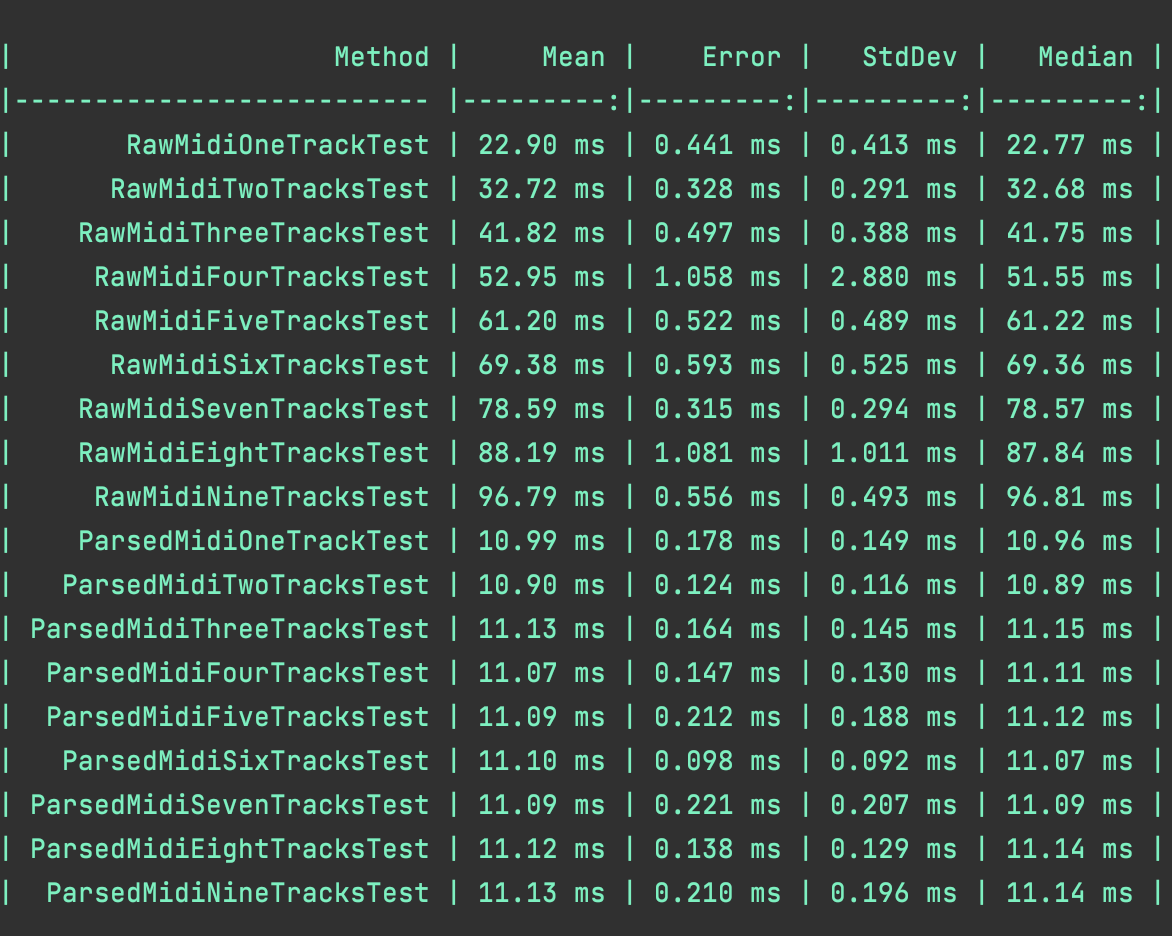
\includegraphics[scale=0.6]{tex/img/FindClean.png}
		
			Рис 4.7 — Сводная таблица работы методов при извлечении из MongoDB
\end{center}

На рисунке 4.8 полученные временные характеристики представлены в графическом виде.

\begin{center}
		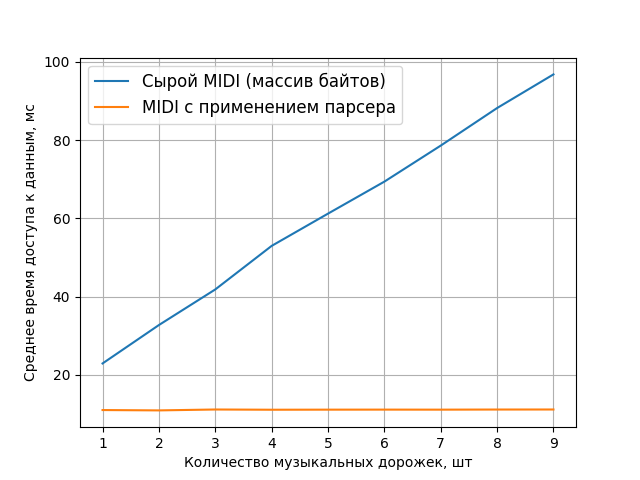
\includegraphics[scale=0.7]{tex/img/figure_find_query.png}
		
			Рис 4.8 — Сравнение работы методов при извлечении из MongoDB
\end{center}

Из рисунков 4.7 и 4.8 видно, что наибольшая скорость выполнения операции чтения документа из MongoDB достигается при использовании метода хранения MIDI-файла в структурированном виде. При этом скорость работы почти не меняется при увеличении числа музыкальных дорожек, разница во времени выполнения доступа к данным при девяти дорожках и одной дорожке составляет 0,14 миллисекунд. Время работы доступа к данным при методе хранения массива байтов, наоборот, растет из-за накладных расходов применяемого парсера. Скорость роста составляет 8,21 мс/шт. Таким образом, реализация хранения в виде структуры MIDI-файла имеет выигрыш по временной эффективности приблизительно в 8,7 раза.

\subsection{Добавление и извлечение документа из MongoDB}

Для оценки времени работы обеих операций добавления и извлечения документов из MongoDB при разных подходах к хранению данных использовались описанные выше методы в совокупности. 
Для исследования добавления и извлечения MIDI-файла, хранящегося в виде струкутры, были использованы методы, представленные на листинге \ref{lst:insert_find_command_test1}. 

\begin{lstlisting}[language=C, label=some-code, caption=Добавление и извлечение MIDI-файла из MongoDB c использованием реализованного метода, label=lst:insert_find_command_test1]
AddDocument("1", "Interstellar1");

var documents = _midiCollection.Find(new BsonDocument()).ToList();
var parsedDocument = documents.Last();

var result =  parsedDocument.GetElement("MTrks").Value.AsBsonArray.Last().AsBsonDocument
    .GetElement("Data").Value.AsByteArray;
\end{lstlisting}

Для исследования добавления и извлечения MIDI-файла, хранящегося в виде массива байтов, были использованы методы, представленные на листинге \ref{lst:insert_find_command_test2}.

\newpage

\begin{lstlisting}[language=C, label=some-code, caption=Добавление и извлечение MIDI-файла из MongoDB в виде массива байтов, label=lst:insert_find_command_test2]

AddBytesMongoDb(FileOperations
    .ReadFileAsync("/Users/anastasia/Interstellar1.mid"));

var documents = _midiCollection.Find(new BsonDocument()).ToList();
var rawDocument = documents.Last();

var midiFileRaw = rawDocument.GetElement("Data").Value.AsByteArray;
var midiFile = _midiFileParser.ParseMidiFile(midiFileRaw);
var result = midiFile.MTrks.Last().Data;
\end{lstlisting}

На рисунке 4.9 представлен результат работы методов хранения. Пояснения исследуемых характеристик приведены на рисунке 4.5.

\begin{center}
		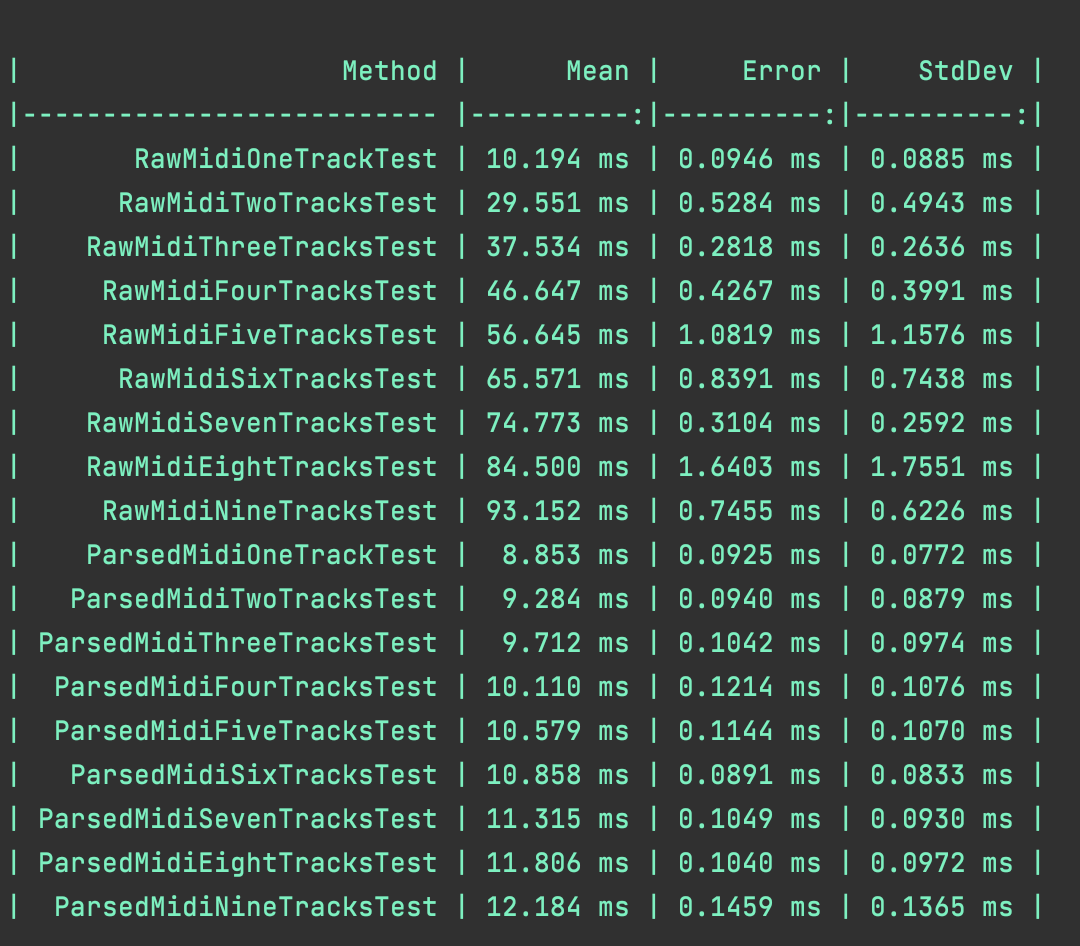
\includegraphics[scale=0.6]{tex/img/InsertFindClean.png}
		
			Рис 4.9 — Сводная таблица работы методов при извлечении из MongoDB
\end{center}

На рисунке 4.10 полученные временные характеристики представлены в графическом виде.

\begin{center}
		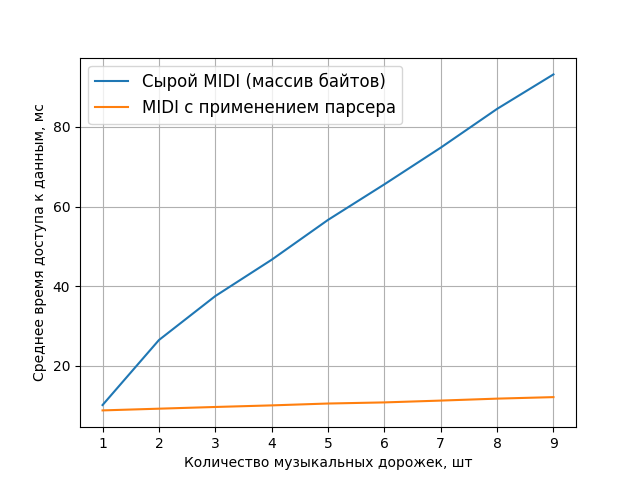
\includegraphics[scale=0.7]{tex/img/figure_find_insert_query.png}
		
			Рис 4.10 — Сравнение работы методов при добавлении и извлечении из MongoDB
\end{center}

Из рисунков 4.9 и 4.10 очевидно, что наибольшая скорость работы операций записи и чтения документа из MongoDB достигается при использовании метода хранения MIDI-файла в структурированном виде. Время работы метода медленно растет при увеличении числа музыкальных дорожек, а скорость роста составляет приблизительно 0,37 мс/шт. Время работы операций записи и чтения при методе хранения массива байтов резко растет, и скорость роста составляет примерно 9,22 мс/шт. Таким образом, реализация хранения MIDI-файла в виде его структуры имеет выигрыш по временной эффективности приблизительно в 7,6 раза. 

\section{Выводы из исследовательского раздела}

В данном разделе было проведено исследование временных характеристик работы операций добавления и извлечения документа из MongoDB при двух способах хранения: с использованием разработанного метода и без использования разработанного метода (хранение в виде массива байтов). По результатам исследования, метод распределенного хранения MIDI-файла в виде его структуры показал немного меньшую эффективность при операции добавления в MongoDB, но значительно большую эффективность при операции извлечения данных, а также при работе обеих этих операций в совокупности. 

%%% Local Variables:
%%% mode: latex
%%% TeX-master: "rpz"
%%% End:
